% Klein bottle square with the horizontal cycle doubled up.
% Source: book/tex/homology/cellular.tex (§ Cellular homology of the Klein bottle).
\documentclass[border=2mm]{standalone}
\usepackage{tikz}
\usepackage{amssymb}
\usetikzlibrary{arrows.meta,decorations.markings}
\tikzset{midarrow/.style={postaction={decorate},decoration={
  markings,mark=at position 0.55 with {\arrow{Latex[length=2mm]}}}}}
\begin{document}
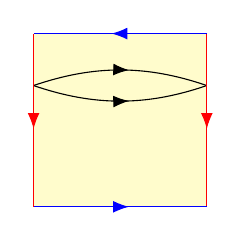
\begin{tikzpicture}[scale=2.2]
  \fill[yellow!20] (0,0) rectangle (1,1);
  \draw[midarrow] (0,0.7) .. controls (0.35,0.82) and (0.65,0.82) .. (1,0.7);
  \draw[midarrow] (0,0.7) .. controls (0.35,0.58) and (0.65,0.58) .. (1,0.7);
  \draw[red, midarrow]  (1,1) -- (1,0);
  \draw[blue, midarrow] (0,0) -- (1,0);
  \draw[red, midarrow]  (0,1) -- (0,0);
  \draw[blue, midarrow] (1,1) -- (0,1);
\end{tikzpicture}
\end{document}
